240. \begin{figure}[ht!]
\center{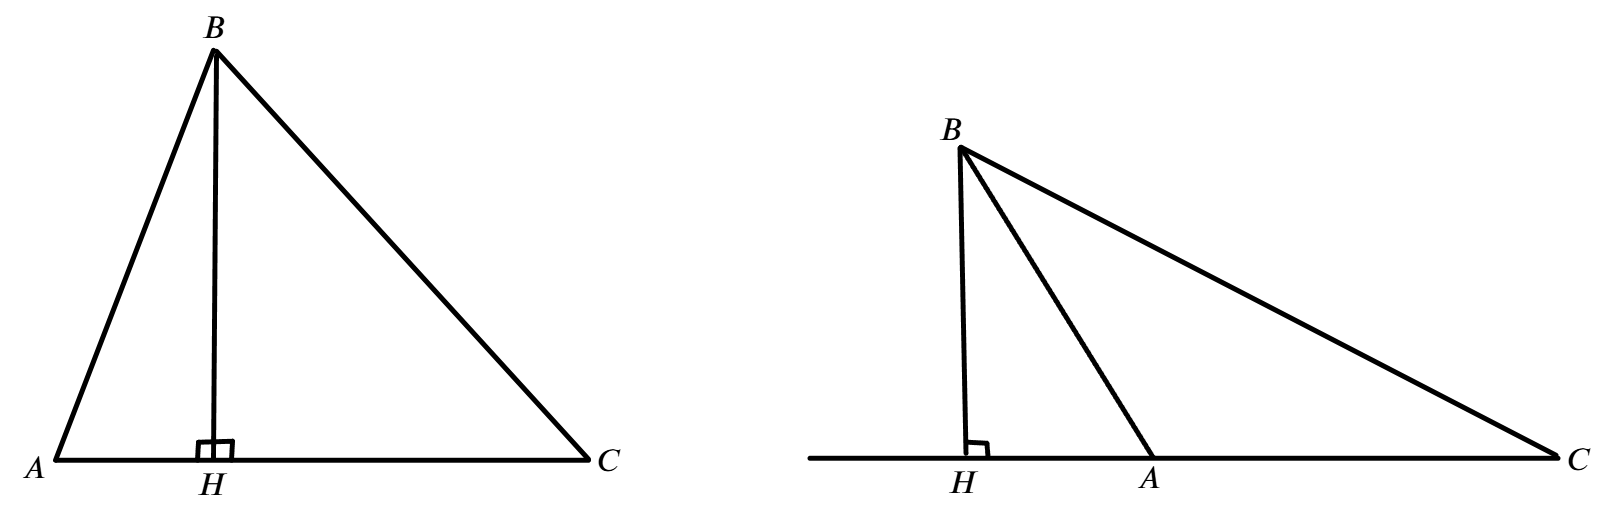
\includegraphics[scale=0.35]{g8-238.png}}
\end{figure}\\
Возможны два случая: треугольник может быть остроугольным или тупоугольным. В первом случае $AH=\sqrt{13^2-12^2}=5,\ CH=\sqrt{15^2-12^2}=9,$ тогда $S=\cfrac{1}{2}\cdot12\cdot(5+9)=84.$ Во втором случае аналогично $S=\cfrac{1}{2}\cdot12\cdot(9-5)=24.$\newpage\noindent
